\chapter{基于 FPGA 的后端加速器详细设计}\label{chap:hardware_design}

本章详细介绍了基于 FPGA 的 SLAM 后端加速器的具体逻辑设计方案。作为全系统的核心，加速器旨在通过深度流水线化和高度并行的存储架构，实现计算密集型算子的高效执行。本章将依次论述总体硬件架构、Jacobi 处理引擎、基于 SOB 编码的动态门控机制、紧凑型存储管理方案以及舒尔消元核心（Schur Core）的实现细节。

\section{总体硬件架构}

针对后端优化算法的计算特性，本文设计了如图~\ref{fig:ba_core_arch} 所示的 Schur Kernel 硬件加速器架构。该架构采用 PS-PL 异构设计：PS 端的 ARM CPU 负责系统控制与参数配置，通过 AXI-Lite 接口与加速器通信；PL 端实现核心计算逻辑，通过 AXI-MM 直接存储器访问（Direct Memory Access, DMA）接口与双倍数据速率（Double Data Rate, DDR）存储器进行高带宽数据交换。加速器内部划分为两个主要计算模块：Jacobi 计算模块和 Schur 消元模块，分别对应 Hessian 构建阶段与边缘化求解阶段。

\begin{figure}[htbp]
    \centering
    \resizebox{0.95\linewidth}{!}{% BA 硬件加速器架构图
% 使用方法: % BA 硬件加速器架构图
% 使用方法: % BA 硬件加速器架构图
% 使用方法: \input{figures/BA_accelerator_arch.tex}
% 符号与论文 main.tex 保持一致
% 字体: 中文使用宋体（继承文档设置），英文使用 Times New Roman（newtxtext）

\begin{tikzpicture}[
    scale=1.0,
    every node/.append style={font=\rmfamily},  % 确保使用衬线字体（Times/宋体）
    % 模块样式
    mainmodule/.style={draw, thick, rounded corners=3pt, minimum width=2.2cm, minimum height=0.7cm, align=center, font=\small},
    submodule/.style={draw, thick, rounded corners=2pt, minimum width=1.8cm, minimum height=0.6cm, align=center, font=\scriptsize},
    buffer/.style={draw, thick, fill=blue!15, minimum width=1.3cm, minimum height=0.5cm, align=center, font=\scriptsize},
    compute/.style={draw, thick, fill=green!15, rounded corners=2pt, minimum width=1.5cm, minimum height=0.5cm, align=center, font=\scriptsize},
    interface/.style={draw, thick, fill=yellow!25, rounded corners=3pt, minimum width=0.8cm, minimum height=1.8cm, align=center, font=\small},
    phasebox/.style={draw, very thick, rounded corners=5pt, fill=#1, fill opacity=0.08},
    arrow/.style={->, >=stealth, thick},
    dataarrow/.style={->, >=stealth, thick, black},
    ctrlarrow/.style={->, >=stealth, dashed, gray},
]

% ========== 外部接口 (左侧竖排) ==========
\node[interface] (ps) at (-1.2, -2.0) {\rotatebox{90}{PS (ARM) CPU}};
\node[interface, fill=orange!20] (ddr) at (-1.2, -6.8) {\rotatebox{90}{DDR Memory}};

% ========== 加速器边框 ==========
\draw[very thick, rounded corners=6pt, fill=gray!5] (0, 0) rectangle (8.5, -9.0);
\node[anchor=north west, font=\bfseries\small] at (0.2, 0) {Schur Kernel Accelerator (PL)};

% ========== AXI 接口 ==========
\node[submodule, fill=yellow!15, minimum width=1.6cm] (axilite) at (1.2, -2.0) {AXI-Lite\\配置接口};
\node[submodule, fill=yellow!15, minimum width=1.6cm] (aximm) at (1.2, -6.8) {AXI-MM\\DMA};

% 外部连接
\draw[arrow] (ps.east) -- (axilite.west);
\draw[<->, thick] (ddr.east) -- (aximm.west);

% ========== 控制单元 ==========
\node[mainmodule, fill=orange!10, minimum width=1.6cm] (ctrl) at (1.2, -3.6) {主控制\\FSM};
\draw[arrow] (axilite.south) -- (ctrl.north);

% ========== Phase 2 区域 ==========
\draw[phasebox=blue!40] (2.4, -0.6) rectangle (8.2, -4.2);
\node[anchor=north west, font=\scriptsize, blue!70] at (2.6, -0.65) {雅可比计算模块};

% Phase 2 输入缓存
\node[buffer] (sob) at (3.5, -1.45) {SOB 解码器};
\node[buffer] (pts) at (5.3, -1.45) {路标点 $\mathbf{L}_j$};
\node[buffer] (feat) at (7.1, -1.45) {观测 $\mathbf{z}_{ij}$};

% 坐标变换
\node[compute, minimum width=4.2cm] (coord) at (5.3, -2.2) {坐标变换: $\mathbf{p}_w \to \mathbf{p}_i \to \mathbf{p}_c$};

% 残差与雅可比
\node[compute, minimum width=1.6cm] (residual) at (3.9, -2.95) {残差 $\mathbf{r}_{ij}$};
\node[compute, minimum width=2cm] (jacobian) at (6.7, -2.95) {雅可比 $\mathbf{J}_p$, $\mathbf{J}_m$};

% Hessian 累积器
\node[compute, minimum width=4.6cm, fill=cyan!15] (accum) at (5.3, -3.75) {Hessian: $\mathbf{H}_{pp}$, $\mathbf{H}_{pm}$, $\mathbf{H}_{mm}$, $\mathbf{b}_p$, $\mathbf{b}_m$};

% Phase 2 内部连接
\draw[dataarrow] (sob.south) -- (3.5, -1.92);
\draw[dataarrow] (pts.south) -- (5.3, -1.92);
\draw[dataarrow] (feat.south) -- (7.1, -1.92);
\draw[dataarrow] (3.9, -2.48) -- (residual.north);
\draw[dataarrow] (6.7, -2.48) -- (jacobian.north);
\draw[dataarrow] (residual.south) -- (3.9, -3.47);
\draw[dataarrow] (jacobian.south) -- (6.7, -3.47);

% ========== 中间缓存 ==========
\node[buffer, minimum width=4.8cm, fill=purple!15] (interbuf) at (5.3, -5.0) {缓存: $\mathbf{H}_{pp}$, $\mathbf{H}_{pm}$, $\mathbf{H}_{mm}$, $\mathbf{b}_p$, $\mathbf{b}_m$};

% Phase 2 到中间缓存
\draw[dataarrow] (accum.south) -- (interbuf.north);

% ========== Phase 3 区域 ==========
\draw[phasebox=red!40] (2.4, -5.8) rectangle (8.2, -8.1);
\node[anchor=north west, font=\scriptsize, red!70] at (2.6, -5.75) {Schur 消元模块};

% Phase 3 计算模块
\node[compute, fill=red!15, minimum width=1.4cm] (vinv) at (3.5, -6.6) {$\mathbf{H}_{mm}^{-1}$};
\node[compute, fill=red!15, minimum width=1.5cm] (wv) at (5.3, -6.6) {$\mathbf{H}_{pm}\mathbf{H}_{mm}^{-1}$};
\node[compute, fill=red!15, minimum width=1.4cm] (schur) at (7.1, -6.6) {$\mathbf{H}_{pp}$ 更新};

% 输出
\node[buffer, minimum width=4.8cm, fill=green!20] (output) at (5.3, -7.55) {输出: $\mathbf{H}_{pp} - \mathbf{H}_{pm}\mathbf{H}_{mm}^{-1}\mathbf{H}_{pm}^T$};

% Phase 3 内部连接
\draw[dataarrow] (vinv.east) -- (wv.west);
\draw[dataarrow] (wv.east) -- (schur.west);
\draw[dataarrow] (schur.south) -- (7.1, -7.22);

% 中间缓存到 Phase 3
\draw[dataarrow] (interbuf.south) -- (5.3, -5.8);

% ========== DMA 数据流 ==========
% DMA 读取到 Phase 2
\draw[dataarrow] (aximm.east) -- (2.2, -6.8) -- (2.2, -1.45) -- (sob.west);

% 输出写回 DMA
\draw[dataarrow] (output.west) -- (1.2, -7.55) -- (aximm.south);

% 控制信号
\draw[ctrlarrow] (ctrl.east) -- (2.4, -3.6);
\draw[ctrlarrow] (ctrl.south) -- (1.2, -6.0) -- (2.4, -6.0);

% ========== 图例 ==========
% 通过形状区分: 缓存为直角矩形, 计算单元为圆角矩形
\node[font=\scriptsize\bfseries] at (0.37, -8.65) {图例:};
\node[draw, thick, minimum width=0.7cm, minimum height=0.3cm] at (1.3, -8.65) {};
\node[font=\tiny, anchor=west] at (1.7, -8.65) {缓存};
\node[draw, thick, rounded corners=2pt, minimum width=0.7cm, minimum height=0.3cm] at (3.2, -8.65) {};
\node[font=\tiny, anchor=west] at (3.6, -8.65) {计算单元};
\draw[->, >=stealth, thick, black] (5.0, -8.65) -- (5.6, -8.65);
\node[font=\tiny, anchor=west] at (5.7, -8.65) {数据流};
\draw[->, >=stealth, dashed, gray] (6.8, -8.65) -- (7.4, -8.65);
\node[font=\tiny, anchor=west] at (7.5, -8.65) {控制};

\end{tikzpicture}

% 符号与论文 main.tex 保持一致
% 字体: 中文使用宋体（继承文档设置），英文使用 Times New Roman（newtxtext）

\begin{tikzpicture}[
    scale=1.0,
    every node/.append style={font=\rmfamily},  % 确保使用衬线字体（Times/宋体）
    % 模块样式
    mainmodule/.style={draw, thick, rounded corners=3pt, minimum width=2.2cm, minimum height=0.7cm, align=center, font=\small},
    submodule/.style={draw, thick, rounded corners=2pt, minimum width=1.8cm, minimum height=0.6cm, align=center, font=\scriptsize},
    buffer/.style={draw, thick, fill=blue!15, minimum width=1.3cm, minimum height=0.5cm, align=center, font=\scriptsize},
    compute/.style={draw, thick, fill=green!15, rounded corners=2pt, minimum width=1.5cm, minimum height=0.5cm, align=center, font=\scriptsize},
    interface/.style={draw, thick, fill=yellow!25, rounded corners=3pt, minimum width=0.8cm, minimum height=1.8cm, align=center, font=\small},
    phasebox/.style={draw, very thick, rounded corners=5pt, fill=#1, fill opacity=0.08},
    arrow/.style={->, >=stealth, thick},
    dataarrow/.style={->, >=stealth, thick, black},
    ctrlarrow/.style={->, >=stealth, dashed, gray},
]

% ========== 外部接口 (左侧竖排) ==========
\node[interface] (ps) at (-1.2, -2.0) {\rotatebox{90}{PS (ARM) CPU}};
\node[interface, fill=orange!20] (ddr) at (-1.2, -6.8) {\rotatebox{90}{DDR Memory}};

% ========== 加速器边框 ==========
\draw[very thick, rounded corners=6pt, fill=gray!5] (0, 0) rectangle (8.5, -9.0);
\node[anchor=north west, font=\bfseries\small] at (0.2, 0) {Schur Kernel Accelerator (PL)};

% ========== AXI 接口 ==========
\node[submodule, fill=yellow!15, minimum width=1.6cm] (axilite) at (1.2, -2.0) {AXI-Lite\\配置接口};
\node[submodule, fill=yellow!15, minimum width=1.6cm] (aximm) at (1.2, -6.8) {AXI-MM\\DMA};

% 外部连接
\draw[arrow] (ps.east) -- (axilite.west);
\draw[<->, thick] (ddr.east) -- (aximm.west);

% ========== 控制单元 ==========
\node[mainmodule, fill=orange!10, minimum width=1.6cm] (ctrl) at (1.2, -3.6) {主控制\\FSM};
\draw[arrow] (axilite.south) -- (ctrl.north);

% ========== Phase 2 区域 ==========
\draw[phasebox=blue!40] (2.4, -0.6) rectangle (8.2, -4.2);
\node[anchor=north west, font=\scriptsize, blue!70] at (2.6, -0.65) {雅可比计算模块};

% Phase 2 输入缓存
\node[buffer] (sob) at (3.5, -1.45) {SOB 解码器};
\node[buffer] (pts) at (5.3, -1.45) {路标点 $\mathbf{L}_j$};
\node[buffer] (feat) at (7.1, -1.45) {观测 $\mathbf{z}_{ij}$};

% 坐标变换
\node[compute, minimum width=4.2cm] (coord) at (5.3, -2.2) {坐标变换: $\mathbf{p}_w \to \mathbf{p}_i \to \mathbf{p}_c$};

% 残差与雅可比
\node[compute, minimum width=1.6cm] (residual) at (3.9, -2.95) {残差 $\mathbf{r}_{ij}$};
\node[compute, minimum width=2cm] (jacobian) at (6.7, -2.95) {雅可比 $\mathbf{J}_p$, $\mathbf{J}_m$};

% Hessian 累积器
\node[compute, minimum width=4.6cm, fill=cyan!15] (accum) at (5.3, -3.75) {Hessian: $\mathbf{H}_{pp}$, $\mathbf{H}_{pm}$, $\mathbf{H}_{mm}$, $\mathbf{b}_p$, $\mathbf{b}_m$};

% Phase 2 内部连接
\draw[dataarrow] (sob.south) -- (3.5, -1.92);
\draw[dataarrow] (pts.south) -- (5.3, -1.92);
\draw[dataarrow] (feat.south) -- (7.1, -1.92);
\draw[dataarrow] (3.9, -2.48) -- (residual.north);
\draw[dataarrow] (6.7, -2.48) -- (jacobian.north);
\draw[dataarrow] (residual.south) -- (3.9, -3.47);
\draw[dataarrow] (jacobian.south) -- (6.7, -3.47);

% ========== 中间缓存 ==========
\node[buffer, minimum width=4.8cm, fill=purple!15] (interbuf) at (5.3, -5.0) {缓存: $\mathbf{H}_{pp}$, $\mathbf{H}_{pm}$, $\mathbf{H}_{mm}$, $\mathbf{b}_p$, $\mathbf{b}_m$};

% Phase 2 到中间缓存
\draw[dataarrow] (accum.south) -- (interbuf.north);

% ========== Phase 3 区域 ==========
\draw[phasebox=red!40] (2.4, -5.8) rectangle (8.2, -8.1);
\node[anchor=north west, font=\scriptsize, red!70] at (2.6, -5.75) {Schur 消元模块};

% Phase 3 计算模块
\node[compute, fill=red!15, minimum width=1.4cm] (vinv) at (3.5, -6.6) {$\mathbf{H}_{mm}^{-1}$};
\node[compute, fill=red!15, minimum width=1.5cm] (wv) at (5.3, -6.6) {$\mathbf{H}_{pm}\mathbf{H}_{mm}^{-1}$};
\node[compute, fill=red!15, minimum width=1.4cm] (schur) at (7.1, -6.6) {$\mathbf{H}_{pp}$ 更新};

% 输出
\node[buffer, minimum width=4.8cm, fill=green!20] (output) at (5.3, -7.55) {输出: $\mathbf{H}_{pp} - \mathbf{H}_{pm}\mathbf{H}_{mm}^{-1}\mathbf{H}_{pm}^T$};

% Phase 3 内部连接
\draw[dataarrow] (vinv.east) -- (wv.west);
\draw[dataarrow] (wv.east) -- (schur.west);
\draw[dataarrow] (schur.south) -- (7.1, -7.22);

% 中间缓存到 Phase 3
\draw[dataarrow] (interbuf.south) -- (5.3, -5.8);

% ========== DMA 数据流 ==========
% DMA 读取到 Phase 2
\draw[dataarrow] (aximm.east) -- (2.2, -6.8) -- (2.2, -1.45) -- (sob.west);

% 输出写回 DMA
\draw[dataarrow] (output.west) -- (1.2, -7.55) -- (aximm.south);

% 控制信号
\draw[ctrlarrow] (ctrl.east) -- (2.4, -3.6);
\draw[ctrlarrow] (ctrl.south) -- (1.2, -6.0) -- (2.4, -6.0);

% ========== 图例 ==========
% 通过形状区分: 缓存为直角矩形, 计算单元为圆角矩形
\node[font=\scriptsize\bfseries] at (0.37, -8.65) {图例:};
\node[draw, thick, minimum width=0.7cm, minimum height=0.3cm] at (1.3, -8.65) {};
\node[font=\tiny, anchor=west] at (1.7, -8.65) {缓存};
\node[draw, thick, rounded corners=2pt, minimum width=0.7cm, minimum height=0.3cm] at (3.2, -8.65) {};
\node[font=\tiny, anchor=west] at (3.6, -8.65) {计算单元};
\draw[->, >=stealth, thick, black] (5.0, -8.65) -- (5.6, -8.65);
\node[font=\tiny, anchor=west] at (5.7, -8.65) {数据流};
\draw[->, >=stealth, dashed, gray] (6.8, -8.65) -- (7.4, -8.65);
\node[font=\tiny, anchor=west] at (7.5, -8.65) {控制};

\end{tikzpicture}

% 符号与论文 main.tex 保持一致
% 字体: 中文使用宋体（继承文档设置），英文使用 Times New Roman（newtxtext）

\begin{tikzpicture}[
    scale=1.0,
    every node/.append style={font=\rmfamily},  % 确保使用衬线字体（Times/宋体）
    % 模块样式
    mainmodule/.style={draw, thick, rounded corners=3pt, minimum width=2.2cm, minimum height=0.7cm, align=center, font=\small},
    submodule/.style={draw, thick, rounded corners=2pt, minimum width=1.8cm, minimum height=0.6cm, align=center, font=\scriptsize},
    buffer/.style={draw, thick, fill=blue!15, minimum width=1.3cm, minimum height=0.5cm, align=center, font=\scriptsize},
    compute/.style={draw, thick, fill=green!15, rounded corners=2pt, minimum width=1.5cm, minimum height=0.5cm, align=center, font=\scriptsize},
    interface/.style={draw, thick, fill=yellow!25, rounded corners=3pt, minimum width=0.8cm, minimum height=1.8cm, align=center, font=\small},
    phasebox/.style={draw, very thick, rounded corners=5pt, fill=#1, fill opacity=0.08},
    arrow/.style={->, >=stealth, thick},
    dataarrow/.style={->, >=stealth, thick, black},
    ctrlarrow/.style={->, >=stealth, dashed, gray},
]

% ========== 外部接口 (左侧竖排) ==========
\node[interface] (ps) at (-1.2, -2.0) {\rotatebox{90}{PS (ARM) CPU}};
\node[interface, fill=orange!20] (ddr) at (-1.2, -6.8) {\rotatebox{90}{DDR Memory}};

% ========== 加速器边框 ==========
\draw[very thick, rounded corners=6pt, fill=gray!5] (0, 0) rectangle (8.5, -9.0);
\node[anchor=north west, font=\bfseries\small] at (0.2, 0) {Schur Kernel Accelerator (PL)};

% ========== AXI 接口 ==========
\node[submodule, fill=yellow!15, minimum width=1.6cm] (axilite) at (1.2, -2.0) {AXI-Lite\\配置接口};
\node[submodule, fill=yellow!15, minimum width=1.6cm] (aximm) at (1.2, -6.8) {AXI-MM\\DMA};

% 外部连接
\draw[arrow] (ps.east) -- (axilite.west);
\draw[<->, thick] (ddr.east) -- (aximm.west);

% ========== 控制单元 ==========
\node[mainmodule, fill=orange!10, minimum width=1.6cm] (ctrl) at (1.2, -3.6) {主控制\\FSM};
\draw[arrow] (axilite.south) -- (ctrl.north);

% ========== Phase 2 区域 ==========
\draw[phasebox=blue!40] (2.4, -0.6) rectangle (8.2, -4.2);
\node[anchor=north west, font=\scriptsize, blue!70] at (2.6, -0.65) {雅可比计算模块};

% Phase 2 输入缓存
\node[buffer] (sob) at (3.5, -1.45) {SOB 解码器};
\node[buffer] (pts) at (5.3, -1.45) {路标点 $\mathbf{L}_j$};
\node[buffer] (feat) at (7.1, -1.45) {观测 $\mathbf{z}_{ij}$};

% 坐标变换
\node[compute, minimum width=4.2cm] (coord) at (5.3, -2.2) {坐标变换: $\mathbf{p}_w \to \mathbf{p}_i \to \mathbf{p}_c$};

% 残差与雅可比
\node[compute, minimum width=1.6cm] (residual) at (3.9, -2.95) {残差 $\mathbf{r}_{ij}$};
\node[compute, minimum width=2cm] (jacobian) at (6.7, -2.95) {雅可比 $\mathbf{J}_p$, $\mathbf{J}_m$};

% Hessian 累积器
\node[compute, minimum width=4.6cm, fill=cyan!15] (accum) at (5.3, -3.75) {Hessian: $\mathbf{H}_{pp}$, $\mathbf{H}_{pm}$, $\mathbf{H}_{mm}$, $\mathbf{b}_p$, $\mathbf{b}_m$};

% Phase 2 内部连接
\draw[dataarrow] (sob.south) -- (3.5, -1.92);
\draw[dataarrow] (pts.south) -- (5.3, -1.92);
\draw[dataarrow] (feat.south) -- (7.1, -1.92);
\draw[dataarrow] (3.9, -2.48) -- (residual.north);
\draw[dataarrow] (6.7, -2.48) -- (jacobian.north);
\draw[dataarrow] (residual.south) -- (3.9, -3.47);
\draw[dataarrow] (jacobian.south) -- (6.7, -3.47);

% ========== 中间缓存 ==========
\node[buffer, minimum width=4.8cm, fill=purple!15] (interbuf) at (5.3, -5.0) {缓存: $\mathbf{H}_{pp}$, $\mathbf{H}_{pm}$, $\mathbf{H}_{mm}$, $\mathbf{b}_p$, $\mathbf{b}_m$};

% Phase 2 到中间缓存
\draw[dataarrow] (accum.south) -- (interbuf.north);

% ========== Phase 3 区域 ==========
\draw[phasebox=red!40] (2.4, -5.8) rectangle (8.2, -8.1);
\node[anchor=north west, font=\scriptsize, red!70] at (2.6, -5.75) {Schur 消元模块};

% Phase 3 计算模块
\node[compute, fill=red!15, minimum width=1.4cm] (vinv) at (3.5, -6.6) {$\mathbf{H}_{mm}^{-1}$};
\node[compute, fill=red!15, minimum width=1.5cm] (wv) at (5.3, -6.6) {$\mathbf{H}_{pm}\mathbf{H}_{mm}^{-1}$};
\node[compute, fill=red!15, minimum width=1.4cm] (schur) at (7.1, -6.6) {$\mathbf{H}_{pp}$ 更新};

% 输出
\node[buffer, minimum width=4.8cm, fill=green!20] (output) at (5.3, -7.55) {输出: $\mathbf{H}_{pp} - \mathbf{H}_{pm}\mathbf{H}_{mm}^{-1}\mathbf{H}_{pm}^T$};

% Phase 3 内部连接
\draw[dataarrow] (vinv.east) -- (wv.west);
\draw[dataarrow] (wv.east) -- (schur.west);
\draw[dataarrow] (schur.south) -- (7.1, -7.22);

% 中间缓存到 Phase 3
\draw[dataarrow] (interbuf.south) -- (5.3, -5.8);

% ========== DMA 数据流 ==========
% DMA 读取到 Phase 2
\draw[dataarrow] (aximm.east) -- (2.2, -6.8) -- (2.2, -1.45) -- (sob.west);

% 输出写回 DMA
\draw[dataarrow] (output.west) -- (1.2, -7.55) -- (aximm.south);

% 控制信号
\draw[ctrlarrow] (ctrl.east) -- (2.4, -3.6);
\draw[ctrlarrow] (ctrl.south) -- (1.2, -6.0) -- (2.4, -6.0);

% ========== 图例 ==========
% 通过形状区分: 缓存为直角矩形, 计算单元为圆角矩形
\node[font=\scriptsize\bfseries] at (0.37, -8.65) {图例:};
\node[draw, thick, minimum width=0.7cm, minimum height=0.3cm] at (1.3, -8.65) {};
\node[font=\tiny, anchor=west] at (1.7, -8.65) {缓存};
\node[draw, thick, rounded corners=2pt, minimum width=0.7cm, minimum height=0.3cm] at (3.2, -8.65) {};
\node[font=\tiny, anchor=west] at (3.6, -8.65) {计算单元};
\draw[->, >=stealth, thick, black] (5.0, -8.65) -- (5.6, -8.65);
\node[font=\tiny, anchor=west] at (5.7, -8.65) {数据流};
\draw[->, >=stealth, dashed, gray] (6.8, -8.65) -- (7.4, -8.65);
\node[font=\tiny, anchor=west] at (7.5, -8.65) {控制};

\end{tikzpicture}
}
    \bicaption{Schur Kernel 硬件加速器架构}{Architecture of Schur Kernel Hardware Accelerator}
    \label{fig:ba_core_arch}
\end{figure}

\begin{enumerate}
    \item \textbf{Jacobi 计算模块}：如图~\ref{fig:ba_core_arch} 上半部分所示，该模块集成了从原始观测数据到 Hessian 矩阵构建的完整计算流程，主要包含以下子单元：
    \begin{itemize}
        \item \textbf{SOB 解码器}：解析稀疏观测位图（SOB）编码，实现动态门控以跳过无效观测；
        \item \textbf{坐标变换单元}：执行 $\mathbf{p}_w \to \mathbf{p}_i \to \mathbf{p}_c$ 的级联坐标变换，将世界坐标系下的路标点 $\mathbf{L}_j$ 依次变换到 IMU 坐标系和相机坐标系；
        \item \textbf{残差计算单元}：根据相机坐标 $\mathbf{p}_c$ 和观测 $\mathbf{z}_{ij}$ 计算重投影残差 $\mathbf{r}_{ij}$；
        \item \textbf{雅可比生成单元}：采用链式法则计算位姿雅可比矩阵 $\mathbf{J}_p$ 和路标雅可比矩阵 $\mathbf{J}_m$；
        \item \textbf{Hessian 累积器}：执行雅可比矩阵外积运算，在线累积 $\mathbf{H}_{pp}$、$\mathbf{H}_{pm}$、$\mathbf{H}_{mm}$ 以及梯度向量 $\mathbf{b}_p$、$\mathbf{b}_m$。
    \end{itemize}
    \item \textbf{Schur 消元模块}：如图~\ref{fig:ba_core_arch} 下半部分所示，该模块负责将路标点从优化问题中边缘化，输出仅关于位姿的简化系统。其计算流程包含三个流水级：
    \begin{itemize}
        \item \textbf{$\mathbf{H}_{mm}^{-1}$ 计算}：利用 $\mathbf{H}_{mm}$ 的块对角特性，采用解析公式直接计算每个 $3\times3$ 子块的逆；
        \item \textbf{$\mathbf{H}_{pm}\mathbf{H}_{mm}^{-1}$ 计算}：对每个有效的状态-路标关联对，计算中间矩阵积；
        \item \textbf{$\mathbf{H}_{pp}$ 更新}：执行舒尔补累加，输出 $\mathbf{H}_{pp} - \mathbf{H}_{pm}\mathbf{H}_{mm}^{-1}\mathbf{H}_{pm}^{\mathrm{T}}$。
    \end{itemize}
\end{enumerate}

\section{Jacobi 处理引擎设计}

\subsection{模块层次与数据依赖}

为保证流水线的高吞吐与低延迟，硬件设计首先明确模块之间的数据依赖关系，并据此划分层次结构。图~\ref{fig:data_dependency} 展示了从输入数据到 Hessian 累积、再到 Schur 消元的关键依赖链路：状态四元数与位置、路标点坐标与相机内参共同决定坐标变换结果 $\mathbf{P}_c$，其进一步驱动残差 $\mathbf{r}$ 与雅可比矩阵 $\mathbf{J}_p, \mathbf{J}_m$ 的生成；在此基础上累积 $\mathbf{A}, \mathbf{b}, \mathbf{V}, \mathbf{g}, \mathbf{W}$ 等中间量，待 Phase2 完成后才能进入 Schur 消元阶段。这一依赖关系确保了“观测独立—点内串行—点间并行”的调度原则。

图~\ref{fig:module_hierarchy} 给出了 Schur Kernel 的模块层次结构，从顶层控制到输入缓冲、坐标变换、雅可比计算、Hessian 累积、Schur 消元及输出缓冲，形成清晰的层次化组织。该结构既便于调试，也有利于后续在不同 FPGA 平台上的资源裁剪与复用。

\begin{figure}[htbp]
    \centering
    \resizebox{0.92\linewidth}{!}{% 数据依赖图
% 使用方法: 在主文档中 % 数据依赖图
% 使用方法: 在主文档中 % 数据依赖图
% 使用方法: 在主文档中 \input{figures/data_dependency.tex}
% 字体: 中文使用宋体（继承文档设置），英文使用 Times New Roman（newtxtext）

\begin{tikzpicture}[
    every node/.append style={font=\rmfamily},  % 确保使用衬线字体（Times/宋体）
    data/.style={draw, thick, rounded corners=3pt, fill=blue!10, minimum width=1.8cm, minimum height=0.6cm, align=center, font=\footnotesize},
    proc/.style={draw, thick, rounded corners=3pt, fill=green!15, minimum width=2.2cm, minimum height=0.7cm, align=center, font=\footnotesize},
    output/.style={draw, thick, rounded corners=3pt, fill=orange!15, minimum width=1.5cm, minimum height=0.6cm, align=center, font=\footnotesize},
    final/.style={draw, thick, rounded corners=3pt, fill=red!15, minimum width=2.5cm, minimum height=0.7cm, align=center, font=\footnotesize},
    arrow/.style={->, >=stealth, thick},
    group_box/.style={draw, dashed, thick, rounded corners=5pt},
]

% ========== 输入数据 ==========
\node[data] (state_quat) at (0, 0) {状态姿态\\参数};
\node[data] (state_pos) at (0, -1) {状态位置\\参数};
\node[data] (pts_pw) at (0, -2) {路标点\\世界坐标};
\node[data] (intrin) at (0, -3) {内参\\参数};

\node[group_box, fit=(state_quat)(state_pos)(pts_pw)(intrin), inner sep=5pt] (input_box) {};
\node[anchor=south, font=\scriptsize\bfseries] at (input_box.north) {输入数据};

% ========== 坐标变换 ==========
\node[proc] (coord_trans) at (4, -1.5) {坐标变换\\$\mathbf{P}_w \to \mathbf{P}_c$};

\draw[arrow] (state_quat) -- (coord_trans);
\draw[arrow] (state_pos) -- (coord_trans);
\draw[arrow] (pts_pw) -- (coord_trans);
\draw[arrow] (intrin) -- (coord_trans);

% ========== 残差计算 ==========
\node[output] (Pc) at (7, -1) {$\mathbf{P}_c$};
\node[proc] (residual) at (10, -1) {残差计算};
\node[output] (r) at (13, -1) {$\mathbf{r}$};

\draw[arrow] (coord_trans) -- (Pc);
\draw[arrow] (Pc) -- (residual);
\draw[arrow] (residual) -- (r);

% ========== 雅可比计算 ==========
\node[proc] (jacobian) at (7, -3) {雅可比计算};

\draw[arrow] (Pc) -- (jacobian);
\draw[arrow] (coord_trans) |- (jacobian);

% ========== 雅可比输出 ==========
\node[output] (jx) at (4, -4.5) {$\mathbf{J}_p$};
\node[output] (jf) at (7, -4.5) {$\mathbf{J}_m$};
\node[output] (dr_dpc) at (10, -4.5) {$\frac{\partial r}{\partial p_c}$};

\draw[arrow] (jacobian) -- (jx);
\draw[arrow] (jacobian) -- (jf);
\draw[arrow] (jacobian) -- (dr_dpc);

% ========== Hessian 累积更新 ==========
\node[group_box, minimum width=10cm, minimum height=1.8cm, fill=yellow!5] (hessian_box) at (7, -6.5) {};
\node[anchor=north, font=\scriptsize\bfseries] at (7, -5.7) {Hessian 累积更新};

\node[output] (A) at (3.5, -6.8) {$\mathbf{H}_{pp}$\\(累加)};
\node[output] (b) at (5.5, -6.8) {$\mathbf{b}_p$\\(累加)};
\node[output] (V) at (7.5, -6.8) {$\mathbf{H}_{mm}$\\(累加)};
\node[output] (g) at (9.5, -6.8) {$\mathbf{b}_m$\\(累加)};

\draw[arrow] (jx) -- (A);
\draw[arrow] (jx) -- (b);
\draw[arrow] (r.south) -- ++(0, -1) -| (b);
\draw[arrow] (jf) -- (V);
\draw[arrow] (jf) -- (g);
\draw[arrow] (r.south) -- ++(0, -1) -| (g);

% H_{pm} 矩阵
\node[output] (W) at (11.5, -6.8) {$\mathbf{H}_{pm}$};
\draw[arrow] (jx.south) -- ++(0, -0.5) -| (W);
\draw[arrow] (jf.south) -- ++(0, -0.5) -| (W);

% ========== Schur 消元 ==========
\node[final] (schur) at (7, -8.5) {Schur消元\\等待 Hessian 累积完成};

\draw[arrow] (A) -- (schur);
\draw[arrow] (b) -- (schur);
\draw[arrow] (V) -- (schur);
\draw[arrow] (g) -- (schur);
\draw[arrow] (W) -- (schur);

% ========== 最终输出 ==========
\node[final, fill=green!20] (output) at (7, -10) {$\mathbf{S}, \mathbf{b}'_p$\\(输出)};

\draw[arrow] (schur) -- (output);

\end{tikzpicture}

% 字体: 中文使用宋体（继承文档设置），英文使用 Times New Roman（newtxtext）

\begin{tikzpicture}[
    every node/.append style={font=\rmfamily},  % 确保使用衬线字体（Times/宋体）
    data/.style={draw, thick, rounded corners=3pt, fill=blue!10, minimum width=1.8cm, minimum height=0.6cm, align=center, font=\footnotesize},
    proc/.style={draw, thick, rounded corners=3pt, fill=green!15, minimum width=2.2cm, minimum height=0.7cm, align=center, font=\footnotesize},
    output/.style={draw, thick, rounded corners=3pt, fill=orange!15, minimum width=1.5cm, minimum height=0.6cm, align=center, font=\footnotesize},
    final/.style={draw, thick, rounded corners=3pt, fill=red!15, minimum width=2.5cm, minimum height=0.7cm, align=center, font=\footnotesize},
    arrow/.style={->, >=stealth, thick},
    group_box/.style={draw, dashed, thick, rounded corners=5pt},
]

% ========== 输入数据 ==========
\node[data] (state_quat) at (0, 0) {状态姿态\\参数};
\node[data] (state_pos) at (0, -1) {状态位置\\参数};
\node[data] (pts_pw) at (0, -2) {路标点\\世界坐标};
\node[data] (intrin) at (0, -3) {内参\\参数};

\node[group_box, fit=(state_quat)(state_pos)(pts_pw)(intrin), inner sep=5pt] (input_box) {};
\node[anchor=south, font=\scriptsize\bfseries] at (input_box.north) {输入数据};

% ========== 坐标变换 ==========
\node[proc] (coord_trans) at (4, -1.5) {坐标变换\\$\mathbf{P}_w \to \mathbf{P}_c$};

\draw[arrow] (state_quat) -- (coord_trans);
\draw[arrow] (state_pos) -- (coord_trans);
\draw[arrow] (pts_pw) -- (coord_trans);
\draw[arrow] (intrin) -- (coord_trans);

% ========== 残差计算 ==========
\node[output] (Pc) at (7, -1) {$\mathbf{P}_c$};
\node[proc] (residual) at (10, -1) {残差计算};
\node[output] (r) at (13, -1) {$\mathbf{r}$};

\draw[arrow] (coord_trans) -- (Pc);
\draw[arrow] (Pc) -- (residual);
\draw[arrow] (residual) -- (r);

% ========== 雅可比计算 ==========
\node[proc] (jacobian) at (7, -3) {雅可比计算};

\draw[arrow] (Pc) -- (jacobian);
\draw[arrow] (coord_trans) |- (jacobian);

% ========== 雅可比输出 ==========
\node[output] (jx) at (4, -4.5) {$\mathbf{J}_p$};
\node[output] (jf) at (7, -4.5) {$\mathbf{J}_m$};
\node[output] (dr_dpc) at (10, -4.5) {$\frac{\partial r}{\partial p_c}$};

\draw[arrow] (jacobian) -- (jx);
\draw[arrow] (jacobian) -- (jf);
\draw[arrow] (jacobian) -- (dr_dpc);

% ========== Hessian 累积更新 ==========
\node[group_box, minimum width=10cm, minimum height=1.8cm, fill=yellow!5] (hessian_box) at (7, -6.5) {};
\node[anchor=north, font=\scriptsize\bfseries] at (7, -5.7) {Hessian 累积更新};

\node[output] (A) at (3.5, -6.8) {$\mathbf{H}_{pp}$\\(累加)};
\node[output] (b) at (5.5, -6.8) {$\mathbf{b}_p$\\(累加)};
\node[output] (V) at (7.5, -6.8) {$\mathbf{H}_{mm}$\\(累加)};
\node[output] (g) at (9.5, -6.8) {$\mathbf{b}_m$\\(累加)};

\draw[arrow] (jx) -- (A);
\draw[arrow] (jx) -- (b);
\draw[arrow] (r.south) -- ++(0, -1) -| (b);
\draw[arrow] (jf) -- (V);
\draw[arrow] (jf) -- (g);
\draw[arrow] (r.south) -- ++(0, -1) -| (g);

% H_{pm} 矩阵
\node[output] (W) at (11.5, -6.8) {$\mathbf{H}_{pm}$};
\draw[arrow] (jx.south) -- ++(0, -0.5) -| (W);
\draw[arrow] (jf.south) -- ++(0, -0.5) -| (W);

% ========== Schur 消元 ==========
\node[final] (schur) at (7, -8.5) {Schur消元\\等待 Hessian 累积完成};

\draw[arrow] (A) -- (schur);
\draw[arrow] (b) -- (schur);
\draw[arrow] (V) -- (schur);
\draw[arrow] (g) -- (schur);
\draw[arrow] (W) -- (schur);

% ========== 最终输出 ==========
\node[final, fill=green!20] (output) at (7, -10) {$\mathbf{S}, \mathbf{b}'_p$\\(输出)};

\draw[arrow] (schur) -- (output);

\end{tikzpicture}

% 字体: 中文使用宋体（继承文档设置），英文使用 Times New Roman（newtxtext）

\begin{tikzpicture}[
    every node/.append style={font=\rmfamily},  % 确保使用衬线字体（Times/宋体）
    data/.style={draw, thick, rounded corners=3pt, fill=blue!10, minimum width=1.8cm, minimum height=0.6cm, align=center, font=\footnotesize},
    proc/.style={draw, thick, rounded corners=3pt, fill=green!15, minimum width=2.2cm, minimum height=0.7cm, align=center, font=\footnotesize},
    output/.style={draw, thick, rounded corners=3pt, fill=orange!15, minimum width=1.5cm, minimum height=0.6cm, align=center, font=\footnotesize},
    final/.style={draw, thick, rounded corners=3pt, fill=red!15, minimum width=2.5cm, minimum height=0.7cm, align=center, font=\footnotesize},
    arrow/.style={->, >=stealth, thick},
    group_box/.style={draw, dashed, thick, rounded corners=5pt},
]

% ========== 输入数据 ==========
\node[data] (state_quat) at (0, 0) {状态姿态\\参数};
\node[data] (state_pos) at (0, -1) {状态位置\\参数};
\node[data] (pts_pw) at (0, -2) {路标点\\世界坐标};
\node[data] (intrin) at (0, -3) {内参\\参数};

\node[group_box, fit=(state_quat)(state_pos)(pts_pw)(intrin), inner sep=5pt] (input_box) {};
\node[anchor=south, font=\scriptsize\bfseries] at (input_box.north) {输入数据};

% ========== 坐标变换 ==========
\node[proc] (coord_trans) at (4, -1.5) {坐标变换\\$\mathbf{P}_w \to \mathbf{P}_c$};

\draw[arrow] (state_quat) -- (coord_trans);
\draw[arrow] (state_pos) -- (coord_trans);
\draw[arrow] (pts_pw) -- (coord_trans);
\draw[arrow] (intrin) -- (coord_trans);

% ========== 残差计算 ==========
\node[output] (Pc) at (7, -1) {$\mathbf{P}_c$};
\node[proc] (residual) at (10, -1) {残差计算};
\node[output] (r) at (13, -1) {$\mathbf{r}$};

\draw[arrow] (coord_trans) -- (Pc);
\draw[arrow] (Pc) -- (residual);
\draw[arrow] (residual) -- (r);

% ========== 雅可比计算 ==========
\node[proc] (jacobian) at (7, -3) {雅可比计算};

\draw[arrow] (Pc) -- (jacobian);
\draw[arrow] (coord_trans) |- (jacobian);

% ========== 雅可比输出 ==========
\node[output] (jx) at (4, -4.5) {$\mathbf{J}_p$};
\node[output] (jf) at (7, -4.5) {$\mathbf{J}_m$};
\node[output] (dr_dpc) at (10, -4.5) {$\frac{\partial r}{\partial p_c}$};

\draw[arrow] (jacobian) -- (jx);
\draw[arrow] (jacobian) -- (jf);
\draw[arrow] (jacobian) -- (dr_dpc);

% ========== Hessian 累积更新 ==========
\node[group_box, minimum width=10cm, minimum height=1.8cm, fill=yellow!5] (hessian_box) at (7, -6.5) {};
\node[anchor=north, font=\scriptsize\bfseries] at (7, -5.7) {Hessian 累积更新};

\node[output] (A) at (3.5, -6.8) {$\mathbf{H}_{pp}$\\(累加)};
\node[output] (b) at (5.5, -6.8) {$\mathbf{b}_p$\\(累加)};
\node[output] (V) at (7.5, -6.8) {$\mathbf{H}_{mm}$\\(累加)};
\node[output] (g) at (9.5, -6.8) {$\mathbf{b}_m$\\(累加)};

\draw[arrow] (jx) -- (A);
\draw[arrow] (jx) -- (b);
\draw[arrow] (r.south) -- ++(0, -1) -| (b);
\draw[arrow] (jf) -- (V);
\draw[arrow] (jf) -- (g);
\draw[arrow] (r.south) -- ++(0, -1) -| (g);

% H_{pm} 矩阵
\node[output] (W) at (11.5, -6.8) {$\mathbf{H}_{pm}$};
\draw[arrow] (jx.south) -- ++(0, -0.5) -| (W);
\draw[arrow] (jf.south) -- ++(0, -0.5) -| (W);

% ========== Schur 消元 ==========
\node[final] (schur) at (7, -8.5) {Schur消元\\等待 Hessian 累积完成};

\draw[arrow] (A) -- (schur);
\draw[arrow] (b) -- (schur);
\draw[arrow] (V) -- (schur);
\draw[arrow] (g) -- (schur);
\draw[arrow] (W) -- (schur);

% ========== 最终输出 ==========
\node[final, fill=green!20] (output) at (7, -10) {$\mathbf{S}, \mathbf{b}'_p$\\(输出)};

\draw[arrow] (schur) -- (output);

\end{tikzpicture}
}
    \bicaption{Jacobi 计算与 Schur 消元的数据依赖关系}{Data dependency across Jacobian generation and Schur elimination}
    \label{fig:data_dependency}
\end{figure}

\begin{figure}[htbp]
    \centering
    \resizebox{0.88\linewidth}{!}{% 模块层次结构图
% 使用方法: 在主文档中 % 模块层次结构图
% 使用方法: 在主文档中 % 模块层次结构图
% 使用方法: 在主文档中 \input{figures/module_hierarchy.tex}
% 字体: 中文使用宋体（继承文档设置），英文使用 Times New Roman（newtxtext）

\begin{tikzpicture}[
    every node/.append style={font=\rmfamily},  % 确保使用衬线字体（Times/宋体）
    level 1/.style={sibling distance=3.8cm, level distance=1.5cm},
    level 2/.style={sibling distance=1.8cm, level distance=1.3cm},
    level 3/.style={sibling distance=1.5cm, level distance=1.2cm},
    module/.style={draw, thick, rounded corners=2pt, fill=blue!10, minimum width=1.8cm, minimum height=0.6cm, align=center, font=\tiny},
    submodule/.style={draw, rounded corners=2pt, fill=green!10, minimum width=1.4cm, minimum height=0.5cm, align=center, font=\tiny},
    leaf/.style={draw, rounded corners=2pt, fill=yellow!10, minimum width=1.2cm, minimum height=0.4cm, align=center, font=\tiny},
    edge from parent/.style={draw, thick, ->,>=stealth},
]

\node[module, minimum width=3cm, fill=blue!20] (top) {schur\_kernel\_top}
    child {node[module] {axi\_lite\_slave}
        child {node[submodule] {register\_file}}
    }
    child {node[module] {axi\_mm\_master}
        child {node[submodule] {read\_engine}}
        child {node[submodule] {write\_engine}}
    }
    child {node[module] {main\_fsm}}
    child {node[module] {input\_buffer}
        child {node[leaf] {state\_param\_buf}}
        child {node[leaf] {sob\_buf}}
        child {node[leaf] {pts\_pw\_buf}}
        child {node[leaf] {feature\_uv\_buf}}
    }
    child {node[module] {coord\_transform\_unit}
        child {node[leaf] {quat\_mult}}
        child {node[leaf] {quat\_conj}}
        child {node[leaf] {quat\_rotate}}
        child {node[leaf] {quat\_to\_rotmat}}
        child {node[leaf] {mat3x3\_mult}}
    }
    child {node[module] {jacobian\_unit}
        child {node[leaf] {residual\_calc}}
        child {node[leaf] {huber\_scale}}
        child {node[leaf] {dr\_dpc\_calc}}
        child {node[leaf] {dpc\_dpos\_calc}}
        child {node[leaf] {jx\_calc}}
        child {node[leaf] {jf\_calc}}
    }
    child {node[module] {hessian\_accum\_unit}
        child {node[leaf] {jxT\_jx\_accum}}
        child {node[leaf] {jfT\_jf\_accum}}
        child {node[leaf] {jxT\_jf\_store}}
        child {node[leaf] {jxT\_r\_accum}}
        child {node[leaf] {jfT\_r\_accum}}
    }
    child {node[module] {intermediate\_buffer}
        child {node[leaf] {tmp\_amtx\_buf}}
        child {node[leaf] {tmp\_bvct\_buf}}
        child {node[leaf] {tmp\_v\_buf}}
        child {node[leaf] {tmp\_gv\_buf}}
        child {node[leaf] {tmp\_w\_buf}}
    }
    child {node[module] {schur\_elim\_unit}
        child {node[leaf] {mat3x3\_inv}}
        child {node[leaf] {w\_vinv\_mult}}
        child {node[leaf] {wvinv\_wT\_mult}}
        child {node[leaf] {wvinv\_g\_mult}}
        child {node[leaf] {a\_update}}
    }
    child {node[module] {output\_buffer}}
    child {node[module] {fp64\_unit}
        child {node[leaf] {fp64\_add[N]}}
        child {node[leaf] {fp64\_mul[M]}}
        child {node[leaf] {fp64\_div}}
        child {node[leaf] {fp64\_sqrt}}
    };

\end{tikzpicture}

% 字体: 中文使用宋体（继承文档设置），英文使用 Times New Roman（newtxtext）

\begin{tikzpicture}[
    every node/.append style={font=\rmfamily},  % 确保使用衬线字体（Times/宋体）
    level 1/.style={sibling distance=3.8cm, level distance=1.5cm},
    level 2/.style={sibling distance=1.8cm, level distance=1.3cm},
    level 3/.style={sibling distance=1.5cm, level distance=1.2cm},
    module/.style={draw, thick, rounded corners=2pt, fill=blue!10, minimum width=1.8cm, minimum height=0.6cm, align=center, font=\tiny},
    submodule/.style={draw, rounded corners=2pt, fill=green!10, minimum width=1.4cm, minimum height=0.5cm, align=center, font=\tiny},
    leaf/.style={draw, rounded corners=2pt, fill=yellow!10, minimum width=1.2cm, minimum height=0.4cm, align=center, font=\tiny},
    edge from parent/.style={draw, thick, ->,>=stealth},
]

\node[module, minimum width=3cm, fill=blue!20] (top) {schur\_kernel\_top}
    child {node[module] {axi\_lite\_slave}
        child {node[submodule] {register\_file}}
    }
    child {node[module] {axi\_mm\_master}
        child {node[submodule] {read\_engine}}
        child {node[submodule] {write\_engine}}
    }
    child {node[module] {main\_fsm}}
    child {node[module] {input\_buffer}
        child {node[leaf] {state\_param\_buf}}
        child {node[leaf] {sob\_buf}}
        child {node[leaf] {pts\_pw\_buf}}
        child {node[leaf] {feature\_uv\_buf}}
    }
    child {node[module] {coord\_transform\_unit}
        child {node[leaf] {quat\_mult}}
        child {node[leaf] {quat\_conj}}
        child {node[leaf] {quat\_rotate}}
        child {node[leaf] {quat\_to\_rotmat}}
        child {node[leaf] {mat3x3\_mult}}
    }
    child {node[module] {jacobian\_unit}
        child {node[leaf] {residual\_calc}}
        child {node[leaf] {huber\_scale}}
        child {node[leaf] {dr\_dpc\_calc}}
        child {node[leaf] {dpc\_dpos\_calc}}
        child {node[leaf] {jx\_calc}}
        child {node[leaf] {jf\_calc}}
    }
    child {node[module] {hessian\_accum\_unit}
        child {node[leaf] {jxT\_jx\_accum}}
        child {node[leaf] {jfT\_jf\_accum}}
        child {node[leaf] {jxT\_jf\_store}}
        child {node[leaf] {jxT\_r\_accum}}
        child {node[leaf] {jfT\_r\_accum}}
    }
    child {node[module] {intermediate\_buffer}
        child {node[leaf] {tmp\_amtx\_buf}}
        child {node[leaf] {tmp\_bvct\_buf}}
        child {node[leaf] {tmp\_v\_buf}}
        child {node[leaf] {tmp\_gv\_buf}}
        child {node[leaf] {tmp\_w\_buf}}
    }
    child {node[module] {schur\_elim\_unit}
        child {node[leaf] {mat3x3\_inv}}
        child {node[leaf] {w\_vinv\_mult}}
        child {node[leaf] {wvinv\_wT\_mult}}
        child {node[leaf] {wvinv\_g\_mult}}
        child {node[leaf] {a\_update}}
    }
    child {node[module] {output\_buffer}}
    child {node[module] {fp64\_unit}
        child {node[leaf] {fp64\_add[N]}}
        child {node[leaf] {fp64\_mul[M]}}
        child {node[leaf] {fp64\_div}}
        child {node[leaf] {fp64\_sqrt}}
    };

\end{tikzpicture}

% 字体: 中文使用宋体（继承文档设置），英文使用 Times New Roman（newtxtext）

\begin{tikzpicture}[
    every node/.append style={font=\rmfamily},  % 确保使用衬线字体（Times/宋体）
    level 1/.style={sibling distance=3.8cm, level distance=1.5cm},
    level 2/.style={sibling distance=1.8cm, level distance=1.3cm},
    level 3/.style={sibling distance=1.5cm, level distance=1.2cm},
    module/.style={draw, thick, rounded corners=2pt, fill=blue!10, minimum width=1.8cm, minimum height=0.6cm, align=center, font=\tiny},
    submodule/.style={draw, rounded corners=2pt, fill=green!10, minimum width=1.4cm, minimum height=0.5cm, align=center, font=\tiny},
    leaf/.style={draw, rounded corners=2pt, fill=yellow!10, minimum width=1.2cm, minimum height=0.4cm, align=center, font=\tiny},
    edge from parent/.style={draw, thick, ->,>=stealth},
]

\node[module, minimum width=3cm, fill=blue!20] (top) {schur\_kernel\_top}
    child {node[module] {axi\_lite\_slave}
        child {node[submodule] {register\_file}}
    }
    child {node[module] {axi\_mm\_master}
        child {node[submodule] {read\_engine}}
        child {node[submodule] {write\_engine}}
    }
    child {node[module] {main\_fsm}}
    child {node[module] {input\_buffer}
        child {node[leaf] {state\_param\_buf}}
        child {node[leaf] {sob\_buf}}
        child {node[leaf] {pts\_pw\_buf}}
        child {node[leaf] {feature\_uv\_buf}}
    }
    child {node[module] {coord\_transform\_unit}
        child {node[leaf] {quat\_mult}}
        child {node[leaf] {quat\_conj}}
        child {node[leaf] {quat\_rotate}}
        child {node[leaf] {quat\_to\_rotmat}}
        child {node[leaf] {mat3x3\_mult}}
    }
    child {node[module] {jacobian\_unit}
        child {node[leaf] {residual\_calc}}
        child {node[leaf] {huber\_scale}}
        child {node[leaf] {dr\_dpc\_calc}}
        child {node[leaf] {dpc\_dpos\_calc}}
        child {node[leaf] {jx\_calc}}
        child {node[leaf] {jf\_calc}}
    }
    child {node[module] {hessian\_accum\_unit}
        child {node[leaf] {jxT\_jx\_accum}}
        child {node[leaf] {jfT\_jf\_accum}}
        child {node[leaf] {jxT\_jf\_store}}
        child {node[leaf] {jxT\_r\_accum}}
        child {node[leaf] {jfT\_r\_accum}}
    }
    child {node[module] {intermediate\_buffer}
        child {node[leaf] {tmp\_amtx\_buf}}
        child {node[leaf] {tmp\_bvct\_buf}}
        child {node[leaf] {tmp\_v\_buf}}
        child {node[leaf] {tmp\_gv\_buf}}
        child {node[leaf] {tmp\_w\_buf}}
    }
    child {node[module] {schur\_elim\_unit}
        child {node[leaf] {mat3x3\_inv}}
        child {node[leaf] {w\_vinv\_mult}}
        child {node[leaf] {wvinv\_wT\_mult}}
        child {node[leaf] {wvinv\_g\_mult}}
        child {node[leaf] {a\_update}}
    }
    child {node[module] {output\_buffer}}
    child {node[module] {fp64\_unit}
        child {node[leaf] {fp64\_add[N]}}
        child {node[leaf] {fp64\_mul[M]}}
        child {node[leaf] {fp64\_div}}
        child {node[leaf] {fp64\_sqrt}}
    };

\end{tikzpicture}
}
    \bicaption{Schur Kernel 硬件模块层次结构}{Module hierarchy of the Schur Kernel accelerator}
    \label{fig:module_hierarchy}
\end{figure}

Jacobi 矩阵的生成是后端优化中计算量最大的环节之一。在本系统中，Jacobi 处理引擎（JPE）负责计算视觉观测残差 $\mathbf{r}$ 对载体位姿 $\mathbf{p}$ 和路标点坐标 $\mathbf{m}$ 的偏导数。为实现高吞吐率与低延迟，JPE 采用 5 级深度流水线并行处理，同时在输入侧与 SOB 解码器耦合，形成“观测判定—流水计算—稀疏累加”的完整数据通路。

\subsection{5 级流水线架构}

雅可比偏导数的计算涉及复杂的坐标系转换与链式法则求导。为最大化吞吐量，JPE 采用 5 级深度流水线架构，通过时间交叠方式同时处理多组观测，显著提升计算效率。各级功能详解如下（对应观测处理流水线如图~\ref{fig:obs_pipeline} 所示）：

\begin{itemize}
    \item \textbf{Stage 1：IMU 坐标系变换与预计算级}。包含两条并行逻辑：(A) 通过坐标差分与四元数旋转电路，将世界坐标系下的路标点 $\mathbf{p}_w$ 变换为 IMU 坐标系下的坐标 $\mathbf{p}_i = \mathbf{q}_{st} \otimes (\mathbf{p}_w - \mathbf{t}_{st})$，其中 $\mathbf{q}_{st}$ 与 $\mathbf{t}_{st}$ 分别为待优化状态位姿的旋转四元数与平移向量，$\otimes$ 表示四元数旋转算子；(B) 同步计算状态旋转矩阵 $\mathbf{R}_{st}$、IMU 点的反对称矩阵 $\mathbf{p}_i^{\wedge}$（其中 $(\cdot)^{\wedge}$ 为将三维向量映射为反对称矩阵的算符，用于表示叉积运算）以及相机-世界旋转矩阵 $\mathbf{R}_{cw}$，为后续链式法则提供中间变量。
    \item \textbf{Stage 2：相机坐标系投影与中间矩阵计算级}。利用外参 $(\mathbf{t}_{ic}, \mathbf{q}_{ic})$ 将 IMU 坐标 $\mathbf{p}_i$ 变换为相机坐标系下的坐标 $\mathbf{p}_c$。同时，配置专用矩阵乘法单元，并行计算 $\mathbf{R}_{ic} \mathbf{p}_i^{\wedge} \mathbf{R}_{st}^{\mathrm{T}}$，其中 $\mathbf{R}_{ic}$ 为由外参 $\mathbf{q}_{ic}$ 转换得到的 IMU 到相机的旋转矩阵。这一项是后续求解位姿导数的关键公共因子。
    \item \textbf{Stage 3：链式法则中间导数计算级}。专注于偏导数的分解计算，降低单级逻辑深度以保证高频运行。结合观测特征点坐标 $(u, v)$ 和预测坐标 $\mathbf{p}_c$，分别计算残差关于相机系坐标点的偏导数 $\partial\mathbf{r}/\partial\mathbf{p}_c$ 和相机系坐标点关于状态位姿的偏导数 $\partial\mathbf{p}_c/\partial\mathbf{x}$。
    \item \textbf{Stage 4：雅可比生成级}。作为导数计算的汇聚点，利用 Stage 3 的中间导数与 Stage 1 的 $\mathbf{R}_{cw}$ 进行组合，并行输出重投影误差对状态位姿的雅可比矩阵 $\mathbf{J}_p$ 和对路标点的雅可比矩阵 $\mathbf{J}_m$。
    \item \textbf{Stage 5：海森累加级}。在流水线末端，配置矩阵乘加阵列执行雅可比矩阵的外积运算 $\mathbf{H} = \mathbf{J}^{\mathrm{T}} \mathbf{W} \mathbf{J}$，将结果直接累加到片上缓存（BRAM）对应的 Hessian 子块（$\mathbf{H}_{pp}, \mathbf{H}_{pm}, \mathbf{H}_{mm}$）中。
\end{itemize}

\subsection{定点化精度优化}

由于 FPGA 对浮点运算的支持成本较高，JPE 全面采用了定点数进行计算。通过对 EuRoC 数据集的仿真分析，本文采用了 Q16.16 的定点格式用于中间雅可比项，而对于路标点逆深度等敏感分量采用了更高的精度保护。实验表明，相比于双精度浮点实现，该定点化方案引入的位姿估计误差低于 0.5\%。

\section{SOB 编码与动态门控机制实现}

为了最大化能效比，加速器利用了 VIO 系统中观测的天然稀疏性。Hessian 矩阵的 $\mathbf{H}_{pm}$ 子块呈现高度不规则的稀疏结构，这源于观测的局部性——一个路标点仅被滑动窗口内少数相机观测到。传统稠密矩阵存储会导致大量零元素占用资源；而通用的 CSR（压缩稀疏行）格式虽能节省存储，但其复杂的索引数组解析会显著增加硬件控制的复杂度与延迟。为此，本系统引入稀疏观测位图（Sparse Observation Bitmap, SOB）编码，将观测拓扑压缩为定长位图，通过位运算直接驱动流水线调度与门控控制。

\subsection{SOB 位定义与编码格式}

本文采用 8 位 SOB 向量对单个路标点在滑动窗口内的观测活跃情况进行编码。设窗口内包含 4 个状态（从旧到新编号为 State 0$\sim$3，对应 $S_1$--$S_4$），每个状态对应左右双目两路观测，则 SOB 位序定义为：
\begin{equation}
    \text{SOB} = [b_7,b_6,b_5,b_4,b_3,b_2,b_1,b_0]
\end{equation}
位序映射关系为：Bit [7:6] $\rightarrow$ State 3（右目/左目），Bit [5:4] $\rightarrow$ State 2（右目/左目），Bit [3:2] $\rightarrow$ State 1（右目/左目），Bit [1:0] $\rightarrow$ State 0（右目/左目）。比特值为 0 表示无观测（对应 $\mathbf{H}_{pm}$ 中的零子块），比特值为 1 表示有效观测（对应非零的 $6\times3$ 有效块）。该编码与特征点数据包同时传输，使硬件能够在进入 Jacobi 计算前完成零块判定并建立观测拓扑。

\begin{figure}[htbp]
    \centering
    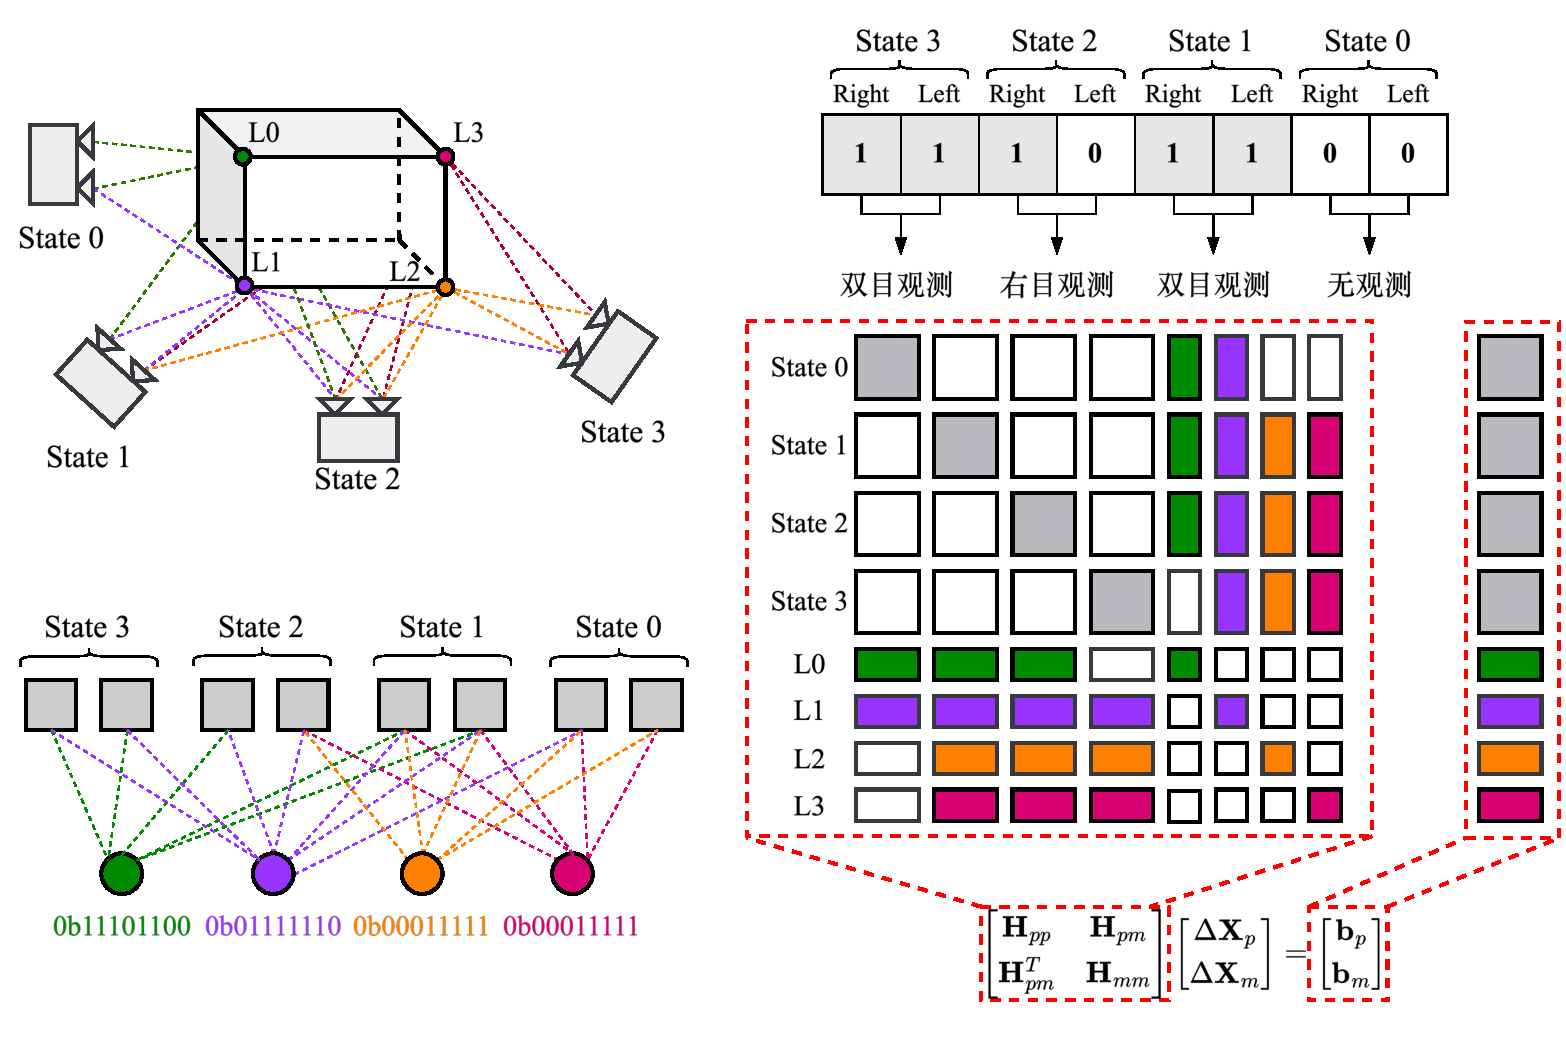
\includegraphics[width=0.78\textwidth]{Img/Observation.pdf}
    \bicaption{稀疏观测位图（SOB）编码示意}{Illustration of Sparse Observation Bitmap (SOB) encoding}
    \label{fig:sob_encoding}
\end{figure}

例如，若某路标点的 SOB 编码为 \texttt{0b11101100}，表示该点仅被 State 1 的双目相机、State 2 的右目相机以及 State 3 的双目相机观测到。在构建 Hessian 矩阵时，系统据此仅对 5 个有效观测开启计算逻辑执行雅可比生成与矩阵累加，而对其余 3 个无效观测（零块）直接执行时钟阻断，从而有效规避不必要的计算开销。

\subsection{SOB 解析逻辑电路}

SOB 解析模块位于 Jacobi 引擎的前端。对于每个传入的路标点包，模块首先提取其携带的 8 位 SOB 正则码，并据此完成观测筛选与流水线调度。观测处理流水线与稀疏累加流程如图~\ref{fig:obs_pipeline} 所示。
\begin{enumerate}
    \item \textbf{高效状态掩码}：通过一组并行的与门（AND Gate）阵列，计算每一位对应的有效性。
    \item \textbf{零块预测器}：当状态对应的两位 $b_{2i+1}$ 和 $b_{2i}$ 均为 0 时，预测器产生一个 \texttt{SKIP\_STATE} 信号。
\end{enumerate}

\begin{figure}[htbp]
    \centering
    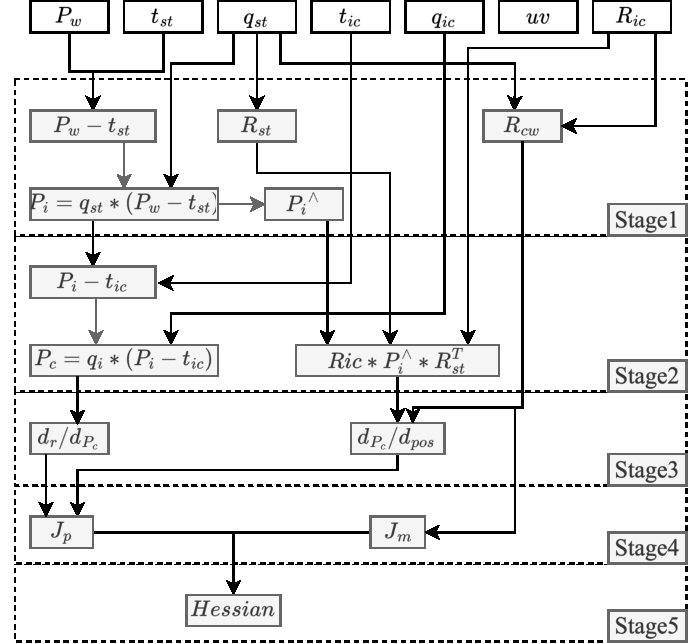
\includegraphics[width=0.86\textwidth]{Img/Hessian-build-pipe.pdf}
    \bicaption{观测处理流水线与稀疏累加流程示意}{Observation processing pipeline and sparse accumulation flow}
    \label{fig:obs_pipeline}
\end{figure}

\subsection{动态时钟门控机制}

为了将稀疏性转化为实际的功耗与速度优势，流水线输入端耦合有稀疏编码解码与判决逻辑。该逻辑根据 SOB 位特征，在硬件底层执行两级动态门控：
\begin{itemize}
    \item \textbf{第一级门控（状态级旁路）}：判决逻辑首先检查代表当前状态（State）的 2 位编码组合（对应左右相机）。若两位均为逻辑“0”（即 \texttt{0b00}），表明该路标点在该时刻完全不可见。此时控制逻辑向 Stage 1 发送旁路信号，直接跳过“世界坐标系到 IMU 坐标系”的刚体变换（包括四元数旋转与平移减法电路），流水线不发生数据翻转。
    \item \textbf{第二级门控（相机级时钟阻断）}：当数据进入后续级数时，判决逻辑进一步检查当前处理相机的独立编码位。若该位为逻辑“0”，表明该特定相机无观测数据。此时控制逻辑向 Stage 2 至 Stage 5 发送时钟门控信号（Clock Gating）：
    \begin{itemize}
        \item \textbf{跳过 Stage 2}：阻断“IMU 系到相机系”的坐标变换及投影计算电路；
        \item \textbf{跳过 Stage 3--4}：阻断雅可比矩阵（$\mathbf{J}_p, \mathbf{J}_m$）的偏导数乘法器时钟；
        \item \textbf{跳过 Stage 5}：阻断 Hessian 矩阵外积（$\mathbf{J}^{\mathrm{T}}\mathbf{J}$）的累加器时钟。
    \end{itemize}
\end{itemize}

为了避免频繁开关时钟造成时序抖动，控制逻辑对 SOB 信号进行了双级寄存器同步，并在状态切换边界插入保护周期（Guard Cycle）。当某一状态的两位均为 0 时，系统不仅跳过该状态的 Jacobi 计算，还会阻断对应 Hessian 块的写入，从而实现“计算—存储”一致的门控策略。通过这种“粗细结合”的门控机制，硬件加速器不仅消除了无效数据的存储访问，更在物理层面完全切断了无效计算路径的动态功耗，实现了计算量与观测稀疏度的线性相关。实验测得在稀疏观测序列中，该机制可降低约 35\% 的动态功耗，如图~\ref{fig:sob_reduction} 所示。

\begin{figure}[htbp]
    \centering
    \resizebox{0.75\textwidth}{!}{% SOB 编码计算量优化效果 - 折线图
% 使用方法: % SOB 编码计算量优化效果 - 折线图
% 使用方法: % SOB 编码计算量优化效果 - 折线图
% 使用方法: \input{figures/sob_computation_chart.tex}
% 字体: 中文使用宋体（继承文档设置），英文使用 Times New Roman（newtxtext）

\usetikzlibrary{arrows.meta}
\begin{tikzpicture}
\begin{axis}[
    every node/.append style={font=\rmfamily},  % 确保使用衬线字体（Times/宋体）
    width=0.85\linewidth,
    height=5.5cm,
    xlabel={稀疏率 (\%)},
    ylabel={迭代次数},
    xmin=30, xmax=80,
    ymin=0, ymax=2200,
    xtick={37.5, 50, 62.5, 73.2},
    legend pos=north west,
    legend style={font=\small},
    grid=major,
    grid style={dashed, gray!30},
    axis lines=left,
    xlabel style={font=\small},
    ylabel style={font=\small},
    tick label style={font=\small},
]

% 朴素迭代 - 蓝色实线
\addplot[
    color=blue,
    mark=square*,
    thick,
    mark size=3pt,
] coordinates {
    (37.5, 400)
    (50.0, 1200)
    (62.5, 1600)
    (73.2, 2048)
};
\addlegendentry{朴素迭代}

% 优化迭代 - 红色虚线
\addplot[
    color=red,
    mark=triangle*,
    thick,
    dashed,
    mark size=3pt,
] coordinates {
    (37.5, 152)
    (50.0, 600)
    (62.5, 974)
    (73.2, 1433)
};
\addlegendentry{SOB 优化迭代}

\end{axis}
\end{tikzpicture}

% 字体: 中文使用宋体（继承文档设置），英文使用 Times New Roman（newtxtext）

\usetikzlibrary{arrows.meta}
\begin{tikzpicture}
\begin{axis}[
    every node/.append style={font=\rmfamily},  % 确保使用衬线字体（Times/宋体）
    width=0.85\linewidth,
    height=5.5cm,
    xlabel={稀疏率 (\%)},
    ylabel={迭代次数},
    xmin=30, xmax=80,
    ymin=0, ymax=2200,
    xtick={37.5, 50, 62.5, 73.2},
    legend pos=north west,
    legend style={font=\small},
    grid=major,
    grid style={dashed, gray!30},
    axis lines=left,
    xlabel style={font=\small},
    ylabel style={font=\small},
    tick label style={font=\small},
]

% 朴素迭代 - 蓝色实线
\addplot[
    color=blue,
    mark=square*,
    thick,
    mark size=3pt,
] coordinates {
    (37.5, 400)
    (50.0, 1200)
    (62.5, 1600)
    (73.2, 2048)
};
\addlegendentry{朴素迭代}

% 优化迭代 - 红色虚线
\addplot[
    color=red,
    mark=triangle*,
    thick,
    dashed,
    mark size=3pt,
] coordinates {
    (37.5, 152)
    (50.0, 600)
    (62.5, 974)
    (73.2, 1433)
};
\addlegendentry{SOB 优化迭代}

\end{axis}
\end{tikzpicture}

% 字体: 中文使用宋体（继承文档设置），英文使用 Times New Roman（newtxtext）

\usetikzlibrary{arrows.meta}
\begin{tikzpicture}
\begin{axis}[
    every node/.append style={font=\rmfamily},  % 确保使用衬线字体（Times/宋体）
    width=0.85\linewidth,
    height=5.5cm,
    xlabel={稀疏率 (\%)},
    ylabel={迭代次数},
    xmin=30, xmax=80,
    ymin=0, ymax=2200,
    xtick={37.5, 50, 62.5, 73.2},
    legend pos=north west,
    legend style={font=\small},
    grid=major,
    grid style={dashed, gray!30},
    axis lines=left,
    xlabel style={font=\small},
    ylabel style={font=\small},
    tick label style={font=\small},
]

% 朴素迭代 - 蓝色实线
\addplot[
    color=blue,
    mark=square*,
    thick,
    mark size=3pt,
] coordinates {
    (37.5, 400)
    (50.0, 1200)
    (62.5, 1600)
    (73.2, 2048)
};
\addlegendentry{朴素迭代}

% 优化迭代 - 红色虚线
\addplot[
    color=red,
    mark=triangle*,
    thick,
    dashed,
    mark size=3pt,
] coordinates {
    (37.5, 152)
    (50.0, 600)
    (62.5, 974)
    (73.2, 1433)
};
\addlegendentry{SOB 优化迭代}

\end{axis}
\end{tikzpicture}
}
    \bicaption{SOB 编码带来的计算量优化效果}{Computation reduction achieved by SOB encoding}
    \label{fig:sob_reduction}
\end{figure}

\subsection{数据与索引分离存储}

针对 $\mathbf{H}_{pm}$ 矩阵子块呈现出的高度不规则稀疏特性，传统的块稀疏行（BSR）或压缩稀疏列（CSC）格式\cite{saad2003iterative}需要显式存储大量的行/列索引数组，不仅占用了额外的存储空间，还增加了硬件地址生成单元的逻辑复杂度。为此，本文利用前述的 SOB 编码，提出了一种“隐式索引”存储优化策略，将数据存储与拓扑结构完全解耦：
\begin{itemize}
    \item \textbf{紧凑数据流（Compact Data Stream）}：鉴于有效观测的稀疏性，系统在片上存储器（BRAM/URAM）中开辟连续的存储空间，仅按顺序紧凑存储非零的有效 Hessian 子块（$6\times3$ 维度）。这种存储方式完全摒弃了零元素的物理存储，实现了“数据即满”，最大化了存储资源的利用率与访存带宽。
    \item \textbf{隐式索引流（Implicit Indexing Stream）}：系统不再维护独立的显式索引表，而是直接复用路标点的 SOB 编码作为元数据索引。硬件解码逻辑通过对掩码执行种群计数（Population Count）指令\cite{warren2013hacker}，即可实时计算出当前路标点对应的有效数据块偏移量与总数；通过检测掩码中“1”的位位置，即可动态解析出每个数据块在逻辑上从属的相机位姿行索引。这种设计将复杂的稀疏矩阵索引操作转化为低延迟的位逻辑运算，确保舒尔消元过程中 $\mathbf{H}_{pm}\mathbf{H}_{mm}^{-1}\mathbf{H}_{pm}^{\mathrm{T}}$ 运算的精确行列对齐。
\end{itemize}


\section{存储管理与 BRAM 优化}

在 Zynq 平台上，片上块存储（BRAM）是非常宝贵的硬件资源。本系统的设计目标是将全滑动窗口的 Hessian 矩阵存储开销控制在 80~KB 以内。为此，系统在存储架构上同时采用“稀疏块压缩 + 数据与索引解耦”的策略，并通过双端口与乒乓缓存机制隐藏访存延迟。此外，PL 端通过 AXI-MM 与 DDR 建立高带宽通路，观测输入与 Schur 输出均采用 DMA 流式传输，从而保证流水线与外部存储节拍匹配。

\subsection{紧凑型 Hessian 存储结构}

由于 $\mathbf{H}_{mm}$ 为块对角矩阵且 $\mathbf{H}_{pm}$ 极其稀疏，系统不再存储完整的密集矩阵，而采用紧凑稀疏块存储方式：
\begin{enumerate}
    \item \textbf{非零块打包}：仅为观测活跃的索引分配存储空间。每个有效的 $6\times3$ 子块采用顺序线性布局，避免零块占用物理地址。
    \item \textbf{隐式索引寻址}：利用 SOB 编码的位索引作为存储地址的一部分，消除了显式索引查找表所需的额外 BRAM；同时与前述“隐式索引流”一致，保证数据流与控制流同步。
\end{enumerate}

\subsection{数据对齐与乒乓缓存}

为支撑 Schur 核心模块的高速运行，Hessian 存储器采用双端口（Dual-port）结构，并实现一套乒乓缓存（Ping-pong Buffer）机制。硬件在计算当前路标点的同时，可将上一路标点的中间更新结果写回，从而隐藏存储器访问延迟。与此同时，输入数据流在片上按固定宽度对齐，确保与 DMA 传输和流水线节拍一致，降低仲裁与跨时钟域同步的开销。

\subsection{主控制 FSM 与数据流调度}

为保证“加载—计算—写回”过程稳定有序，加速器内部设计了主控制状态机（FSM），其状态转移与流水线执行关系如图~\ref{fig:main_fsm} 所示。FSM 从 \texttt{IDLE} 状态响应启动信号，依次完成参数加载（\texttt{LOAD\_PARAMS}）、观测与位图并行读取（\texttt{LOAD\_INPUTS}），随后进入 Phase2/Phase3 计算循环，并在完成 Schur 更新后通过 DMA 写回结果，最终回到空闲状态等待下一帧。

\begin{figure}[htbp]
    \centering
    \resizebox{0.88\linewidth}{!}{% 主控制状态机 FSM 图
% 使用方法: 在主文档中 % 主控制状态机 FSM 图
% 使用方法: 在主文档中 % 主控制状态机 FSM 图
% 使用方法: 在主文档中 \input{figures/main_fsm.tex}
% 字体: 中文使用宋体（继承文档设置），英文使用 Times New Roman（newtxtext）

\begin{tikzpicture}[
    every node/.append style={font=\rmfamily},  % 确保使用衬线字体（Times/宋体）
    state/.style={draw, thick, rounded corners=5pt, minimum width=2.6cm, minimum height=0.9cm, align=center, font=\footnotesize},
    state_idle/.style={state, fill=gray!20},
    state_load/.style={state, fill=blue!15},
    state_phase2/.style={state, fill=green!15},
    state_phase3/.style={state, fill=orange!15},
    state_write/.style={state, fill=purple!15},
    state_done/.style={state, fill=yellow!20},
    arrow/.style={->, >=Stealth, thick},
    condition/.style={font=\tiny, align=center},
    loop_box/.style={draw, dashed, thick, rounded corners=8pt, fill=white, fill opacity=0.7},
]

% ========== 状态节点 ==========
\node[state_idle] (idle) at (0, 0) {IDLE};

\node[state_load] (load_param) at (0, -1.8) {LOAD\_PARAMS\\读取参数};

\node[state_load] (load_input) at (0, -3.6) {LOAD\_INPUTS\\读取SOB/观测/路标};

\node[state_phase2] (p2_init) at (0, -5.4) {PHASE2\_INIT\\初始化循环计数器};

% Phase 2 循环框
\node[loop_box, minimum width=6.5cm, minimum height=4.2cm] (p2_loop_box) at (4.5, -7.8) {};
\node[anchor=north, font=\footnotesize\bfseries] at (4.5, -5.8) {PHASE2\_LOOP};

\node[state_phase2] (p2_check) at (4.5, -6.8) {SOB 判定\\(state, cam)有效?};
\node[state_phase2] (coord_trans) at (2.5, -8.2) {COORD\\TRANSFORM};
\node[state_phase2] (residual) at (4.5, -8.2) {RESIDUAL\\CALC};
\node[state_phase2] (jacobian) at (6.5, -8.2) {JACOBIAN\\CALC};
\node[state_phase2] (hessian) at (4.5, -9.4) {HESSIAN\\ACCUM};

\node[state_phase3] (p3_init) at (0, -11) {PHASE3\_INIT\\初始化Schur循环};

% Phase 3 循环框
\node[loop_box, minimum width=6.5cm, minimum height=3.5cm] (p3_loop_box) at (4.5, -12.8) {};
\node[anchor=north, font=\footnotesize\bfseries] at (4.5, -10.9) {PHASE3\_LOOP};

\node[state_phase3] (v_inv) at (2.5, -12) {$\mathbf{H}_{mm}^{-1}$计算\\(j==0)};
\node[state_phase3] (wvinv) at (6.5, -12) {$\mathbf{H}_{pm}\mathbf{H}_{mm}^{-1}$\\计算};
\node[state_phase3] (schur_update) at (4.5, -13.5) {Schur 更新\\$\mathbf{H}_{pp}, \mathbf{b}_p$};

\node[state_write] (write_out) at (0, -15) {WRITE\_OUTPUT\\DMA写回结果};

\node[state_done] (complete) at (0, -16.8) {COMPLETE\\置位ICR.COMPLETE};

% ========== 状态转移 ==========
% IDLE -> LOAD_PARAMS
\draw[arrow] (idle) -- node[right, condition] {IP\_ENABLE\\$\land$ START\_H} (load_param);

% LOAD_PARAMS -> LOAD_INPUTS
\draw[arrow] (load_param) -- node[right, condition] {读取完成} (load_input);

% LOAD_INPUTS -> PHASE2_INIT
\draw[arrow] (load_input) -- node[right, condition] {加载完成} (p2_init);

% PHASE2_INIT -> PHASE2_LOOP
\draw[arrow] (p2_init) -- ++(2, 0) |- (p2_check);

% Phase 2 内部流程
\draw[arrow] (p2_check) -- node[left, condition] {有效} (coord_trans);
\draw[arrow] (coord_trans) -- (residual);
\draw[arrow] (residual) -- (jacobian);
\draw[arrow] (jacobian) -- (hessian);

% Phase 2 跳过路径
\draw[arrow, dashed] (p2_check.east) -- ++(1.5, 0) node[right, condition] {无效\\跳过} |- (hessian.east);

% Phase 2 循环返回
\draw[arrow] (hessian.south) -- ++(0, -0.3) -- ++(3.5, 0) -- ++(0, 3.0) -- ++(-3.5, 0) -- (p2_check.east);
\node[condition] at (8.5, -8) {cam++\\state++\\pt++};

% PHASE2 -> PHASE3_INIT
\draw[arrow] (hessian.west) -- ++(-3, 0) |- node[left, condition, pos=0.75] {pt $\geq$ num\_pts} (p3_init);

% PHASE3_INIT -> PHASE3_LOOP
\draw[arrow] (p3_init) -- ++(2, 0) |- (v_inv);

% Phase 3 内部流程
\draw[arrow] (v_inv) -- (wvinv);
\draw[arrow] (wvinv) -- (schur_update);

% Phase 3 循环返回
\draw[arrow] (schur_update.south) -- ++(0, -0.3) -- ++(3.5, 0) -- ++(0, 2.0) -- ++(-5.5, 0) -- (v_inv.west);
\node[condition] at (8.5, -12.5) {pt++\\j++};

% PHASE3 -> WRITE_OUTPUT
\draw[arrow] (schur_update.west) -- ++(-3, 0) |- node[left, condition, pos=0.8] {j $\geq$ state\_size} (write_out);

% WRITE_OUTPUT -> COMPLETE
\draw[arrow] (write_out) -- node[right, condition] {写入完成} (complete);

% COMPLETE -> IDLE (返回)
\draw[arrow] (complete.west) -- ++(-2, 0) -- ++(0, 16.8) -- (idle.west);

\end{tikzpicture}

% 字体: 中文使用宋体（继承文档设置），英文使用 Times New Roman（newtxtext）

\begin{tikzpicture}[
    every node/.append style={font=\rmfamily},  % 确保使用衬线字体（Times/宋体）
    state/.style={draw, thick, rounded corners=5pt, minimum width=2.6cm, minimum height=0.9cm, align=center, font=\footnotesize},
    state_idle/.style={state, fill=gray!20},
    state_load/.style={state, fill=blue!15},
    state_phase2/.style={state, fill=green!15},
    state_phase3/.style={state, fill=orange!15},
    state_write/.style={state, fill=purple!15},
    state_done/.style={state, fill=yellow!20},
    arrow/.style={->, >=Stealth, thick},
    condition/.style={font=\tiny, align=center},
    loop_box/.style={draw, dashed, thick, rounded corners=8pt, fill=white, fill opacity=0.7},
]

% ========== 状态节点 ==========
\node[state_idle] (idle) at (0, 0) {IDLE};

\node[state_load] (load_param) at (0, -1.8) {LOAD\_PARAMS\\读取参数};

\node[state_load] (load_input) at (0, -3.6) {LOAD\_INPUTS\\读取SOB/观测/路标};

\node[state_phase2] (p2_init) at (0, -5.4) {PHASE2\_INIT\\初始化循环计数器};

% Phase 2 循环框
\node[loop_box, minimum width=6.5cm, minimum height=4.2cm] (p2_loop_box) at (4.5, -7.8) {};
\node[anchor=north, font=\footnotesize\bfseries] at (4.5, -5.8) {PHASE2\_LOOP};

\node[state_phase2] (p2_check) at (4.5, -6.8) {SOB 判定\\(state, cam)有效?};
\node[state_phase2] (coord_trans) at (2.5, -8.2) {COORD\\TRANSFORM};
\node[state_phase2] (residual) at (4.5, -8.2) {RESIDUAL\\CALC};
\node[state_phase2] (jacobian) at (6.5, -8.2) {JACOBIAN\\CALC};
\node[state_phase2] (hessian) at (4.5, -9.4) {HESSIAN\\ACCUM};

\node[state_phase3] (p3_init) at (0, -11) {PHASE3\_INIT\\初始化Schur循环};

% Phase 3 循环框
\node[loop_box, minimum width=6.5cm, minimum height=3.5cm] (p3_loop_box) at (4.5, -12.8) {};
\node[anchor=north, font=\footnotesize\bfseries] at (4.5, -10.9) {PHASE3\_LOOP};

\node[state_phase3] (v_inv) at (2.5, -12) {$\mathbf{H}_{mm}^{-1}$计算\\(j==0)};
\node[state_phase3] (wvinv) at (6.5, -12) {$\mathbf{H}_{pm}\mathbf{H}_{mm}^{-1}$\\计算};
\node[state_phase3] (schur_update) at (4.5, -13.5) {Schur 更新\\$\mathbf{H}_{pp}, \mathbf{b}_p$};

\node[state_write] (write_out) at (0, -15) {WRITE\_OUTPUT\\DMA写回结果};

\node[state_done] (complete) at (0, -16.8) {COMPLETE\\置位ICR.COMPLETE};

% ========== 状态转移 ==========
% IDLE -> LOAD_PARAMS
\draw[arrow] (idle) -- node[right, condition] {IP\_ENABLE\\$\land$ START\_H} (load_param);

% LOAD_PARAMS -> LOAD_INPUTS
\draw[arrow] (load_param) -- node[right, condition] {读取完成} (load_input);

% LOAD_INPUTS -> PHASE2_INIT
\draw[arrow] (load_input) -- node[right, condition] {加载完成} (p2_init);

% PHASE2_INIT -> PHASE2_LOOP
\draw[arrow] (p2_init) -- ++(2, 0) |- (p2_check);

% Phase 2 内部流程
\draw[arrow] (p2_check) -- node[left, condition] {有效} (coord_trans);
\draw[arrow] (coord_trans) -- (residual);
\draw[arrow] (residual) -- (jacobian);
\draw[arrow] (jacobian) -- (hessian);

% Phase 2 跳过路径
\draw[arrow, dashed] (p2_check.east) -- ++(1.5, 0) node[right, condition] {无效\\跳过} |- (hessian.east);

% Phase 2 循环返回
\draw[arrow] (hessian.south) -- ++(0, -0.3) -- ++(3.5, 0) -- ++(0, 3.0) -- ++(-3.5, 0) -- (p2_check.east);
\node[condition] at (8.5, -8) {cam++\\state++\\pt++};

% PHASE2 -> PHASE3_INIT
\draw[arrow] (hessian.west) -- ++(-3, 0) |- node[left, condition, pos=0.75] {pt $\geq$ num\_pts} (p3_init);

% PHASE3_INIT -> PHASE3_LOOP
\draw[arrow] (p3_init) -- ++(2, 0) |- (v_inv);

% Phase 3 内部流程
\draw[arrow] (v_inv) -- (wvinv);
\draw[arrow] (wvinv) -- (schur_update);

% Phase 3 循环返回
\draw[arrow] (schur_update.south) -- ++(0, -0.3) -- ++(3.5, 0) -- ++(0, 2.0) -- ++(-5.5, 0) -- (v_inv.west);
\node[condition] at (8.5, -12.5) {pt++\\j++};

% PHASE3 -> WRITE_OUTPUT
\draw[arrow] (schur_update.west) -- ++(-3, 0) |- node[left, condition, pos=0.8] {j $\geq$ state\_size} (write_out);

% WRITE_OUTPUT -> COMPLETE
\draw[arrow] (write_out) -- node[right, condition] {写入完成} (complete);

% COMPLETE -> IDLE (返回)
\draw[arrow] (complete.west) -- ++(-2, 0) -- ++(0, 16.8) -- (idle.west);

\end{tikzpicture}

% 字体: 中文使用宋体（继承文档设置），英文使用 Times New Roman（newtxtext）

\begin{tikzpicture}[
    every node/.append style={font=\rmfamily},  % 确保使用衬线字体（Times/宋体）
    state/.style={draw, thick, rounded corners=5pt, minimum width=2.6cm, minimum height=0.9cm, align=center, font=\footnotesize},
    state_idle/.style={state, fill=gray!20},
    state_load/.style={state, fill=blue!15},
    state_phase2/.style={state, fill=green!15},
    state_phase3/.style={state, fill=orange!15},
    state_write/.style={state, fill=purple!15},
    state_done/.style={state, fill=yellow!20},
    arrow/.style={->, >=Stealth, thick},
    condition/.style={font=\tiny, align=center},
    loop_box/.style={draw, dashed, thick, rounded corners=8pt, fill=white, fill opacity=0.7},
]

% ========== 状态节点 ==========
\node[state_idle] (idle) at (0, 0) {IDLE};

\node[state_load] (load_param) at (0, -1.8) {LOAD\_PARAMS\\读取参数};

\node[state_load] (load_input) at (0, -3.6) {LOAD\_INPUTS\\读取SOB/观测/路标};

\node[state_phase2] (p2_init) at (0, -5.4) {PHASE2\_INIT\\初始化循环计数器};

% Phase 2 循环框
\node[loop_box, minimum width=6.5cm, minimum height=4.2cm] (p2_loop_box) at (4.5, -7.8) {};
\node[anchor=north, font=\footnotesize\bfseries] at (4.5, -5.8) {PHASE2\_LOOP};

\node[state_phase2] (p2_check) at (4.5, -6.8) {SOB 判定\\(state, cam)有效?};
\node[state_phase2] (coord_trans) at (2.5, -8.2) {COORD\\TRANSFORM};
\node[state_phase2] (residual) at (4.5, -8.2) {RESIDUAL\\CALC};
\node[state_phase2] (jacobian) at (6.5, -8.2) {JACOBIAN\\CALC};
\node[state_phase2] (hessian) at (4.5, -9.4) {HESSIAN\\ACCUM};

\node[state_phase3] (p3_init) at (0, -11) {PHASE3\_INIT\\初始化Schur循环};

% Phase 3 循环框
\node[loop_box, minimum width=6.5cm, minimum height=3.5cm] (p3_loop_box) at (4.5, -12.8) {};
\node[anchor=north, font=\footnotesize\bfseries] at (4.5, -10.9) {PHASE3\_LOOP};

\node[state_phase3] (v_inv) at (2.5, -12) {$\mathbf{H}_{mm}^{-1}$计算\\(j==0)};
\node[state_phase3] (wvinv) at (6.5, -12) {$\mathbf{H}_{pm}\mathbf{H}_{mm}^{-1}$\\计算};
\node[state_phase3] (schur_update) at (4.5, -13.5) {Schur 更新\\$\mathbf{H}_{pp}, \mathbf{b}_p$};

\node[state_write] (write_out) at (0, -15) {WRITE\_OUTPUT\\DMA写回结果};

\node[state_done] (complete) at (0, -16.8) {COMPLETE\\置位ICR.COMPLETE};

% ========== 状态转移 ==========
% IDLE -> LOAD_PARAMS
\draw[arrow] (idle) -- node[right, condition] {IP\_ENABLE\\$\land$ START\_H} (load_param);

% LOAD_PARAMS -> LOAD_INPUTS
\draw[arrow] (load_param) -- node[right, condition] {读取完成} (load_input);

% LOAD_INPUTS -> PHASE2_INIT
\draw[arrow] (load_input) -- node[right, condition] {加载完成} (p2_init);

% PHASE2_INIT -> PHASE2_LOOP
\draw[arrow] (p2_init) -- ++(2, 0) |- (p2_check);

% Phase 2 内部流程
\draw[arrow] (p2_check) -- node[left, condition] {有效} (coord_trans);
\draw[arrow] (coord_trans) -- (residual);
\draw[arrow] (residual) -- (jacobian);
\draw[arrow] (jacobian) -- (hessian);

% Phase 2 跳过路径
\draw[arrow, dashed] (p2_check.east) -- ++(1.5, 0) node[right, condition] {无效\\跳过} |- (hessian.east);

% Phase 2 循环返回
\draw[arrow] (hessian.south) -- ++(0, -0.3) -- ++(3.5, 0) -- ++(0, 3.0) -- ++(-3.5, 0) -- (p2_check.east);
\node[condition] at (8.5, -8) {cam++\\state++\\pt++};

% PHASE2 -> PHASE3_INIT
\draw[arrow] (hessian.west) -- ++(-3, 0) |- node[left, condition, pos=0.75] {pt $\geq$ num\_pts} (p3_init);

% PHASE3_INIT -> PHASE3_LOOP
\draw[arrow] (p3_init) -- ++(2, 0) |- (v_inv);

% Phase 3 内部流程
\draw[arrow] (v_inv) -- (wvinv);
\draw[arrow] (wvinv) -- (schur_update);

% Phase 3 循环返回
\draw[arrow] (schur_update.south) -- ++(0, -0.3) -- ++(3.5, 0) -- ++(0, 2.0) -- ++(-5.5, 0) -- (v_inv.west);
\node[condition] at (8.5, -12.5) {pt++\\j++};

% PHASE3 -> WRITE_OUTPUT
\draw[arrow] (schur_update.west) -- ++(-3, 0) |- node[left, condition, pos=0.8] {j $\geq$ state\_size} (write_out);

% WRITE_OUTPUT -> COMPLETE
\draw[arrow] (write_out) -- node[right, condition] {写入完成} (complete);

% COMPLETE -> IDLE (返回)
\draw[arrow] (complete.west) -- ++(-2, 0) -- ++(0, 16.8) -- (idle.west);

\end{tikzpicture}
}
    \bicaption{主控制状态机（FSM）与阶段调度流程}{Main FSM and phase scheduling flow}
    \label{fig:main_fsm}
\end{figure}

在 Phase2 循环中，FSM 根据 SOB 位判断当前 (state, cam) 观测是否有效；若无效则触发旁路路径直接跳至 Hessian 累加阶段并维持门控信号，避免无效计算。Phase3 循环在 $j=0$ 时触发 $\mathbf{H}_{mm}^{-1}$ 求逆，随后计算 $\mathbf{H}_{pm}\mathbf{H}_{mm}^{-1}$ 并进行 Schur 更新。状态机通过计数器管理路标点与状态索引，实现对稀疏结构的顺序遍历与数据复用。

\section{Schur 核心模块实现}

Schur 核心模块是实现路标点消去的关键环节。其核心任务是计算 $\mathbf{S} = \mathbf{H}_{pp} - \mathbf{H}_{pm}\mathbf{H}_{mm}^{-1}\mathbf{H}_{pm}^{\top}$。需要说明的是，本文用大写 $\mathbf{H}$ 表示完整的 Hessian 矩阵或其分块，用小写 $\mathbf{h}$ 表示对应于单个路标点或单个状态-路标关联的子块，以便区分全局矩阵与局部子块的计算。

\subsection{并行化 Hmm 求逆器}

针对特征点对应的 $3 \times 3$ 海森矩阵块 $\mathbf{H}_{mm}$，本系统实现了专用的求逆器单元。
\begin{itemize}
    \item \textbf{解析解求逆}：利用海森矩阵的正定对称特性，采用解析解法而非高斯消元法进行 $3 \times 3$ 矩阵求逆。
    \item \textbf{流水化执行}：求逆逻辑内部被划分为 3 个子阶段，支持在单时钟周期内发起多次求逆请求。
\end{itemize}

\subsection{对称 Hessian 更新逻辑}

为了减少 $\mathbf{H}_{pm}\mathbf{H}_{mm}^{-1}\mathbf{H}_{pm}^{\top}$ 计算过程中的乘法器消耗，内核利用了计算结果的对称性（Symmetry）。硬件仅计算 Schur 矩阵 $\mathbf{S}$ 的上三角部分，并通过镜像填充下三角，从而将所需的 DSP 资源和计算周期减半。最终，计算出的压缩 $\mathbf{S}$ 矩阵通过 DMA 通道传输回 PS 端，由 ARM 处理器执行最后的位姿更新。

\subsection{三阶段舒尔消元流水}

舒尔消元模块负责将路标点从优化问题中边缘化，输出仅关于位姿的简化系统。其核心计算按照“求逆—中间积—累加更新”的三阶段流水展开，并在每个阶段复用片上缓存以提升吞吐。

\textbf{（1）路标 Hessian 求逆（$\mathbf{H}_{mm}^{-1}$ 计算）}

由于 $\mathbf{H}_{mm}$ 是块对角矩阵，其中每个对角块 $\mathbf{h}_{mm,k}$ 为对应第 $k$ 个路标点的 $3\times3$ 对称正定矩阵。硬件采用解析公式直接计算每个小矩阵的逆，避免大规模矩阵分解开销。该计算在专用矩阵求逆单元中完成，输出的 $\mathbf{h}_{mm,k}^{-1}$ 被缓存于片上 BRAM 中供后续阶段复用。

\textbf{（2）中间积计算（$\mathbf{h}_{pm,ik}\cdot\mathbf{h}_{mm,k}^{-1}$）}

对于每个有效的“状态-路标”关联对 $(i,k)$（由 SOB 编码指示），硬件计算中间矩阵积 $\mathbf{M}_{ik}=\mathbf{h}_{pm,ik}\cdot\mathbf{h}_{mm,k}^{-1}$。其中 $\mathbf{h}_{pm,ik}$ 为状态 $i$ 与路标 $k$ 之间的 $6\times3$ 交叉项 Hessian 子块。该中间结果 $\mathbf{M}_{ik}$（维度 $6\times3$）被缓存以供下一阶段的梯度和 Hessian 更新复用，避免重复计算。

\textbf{（3）舒尔补累加}

利用缓存的中间积 $\mathbf{M}_{ik}$，硬件并行执行两类累加更新：
\begin{itemize}
    \item \textbf{梯度向量更新}：对于每个有效的状态-路标对 $(i,k)$，计算 $\mathbf{b}_i \leftarrow \mathbf{b}_i - \mathbf{M}_{ik}\cdot\mathbf{g}_k$，其中 $\mathbf{g}_k$ 为路标 $k$ 的 $3\times1$ 梯度向量。
    \item \textbf{Hessian 矩阵更新}：对于所有同时观测到路标 $k$ 的状态对 $(i,j)$，计算 $\mathbf{H}_{pp,ij} \leftarrow \mathbf{H}_{pp,ij} - \mathbf{M}_{ik}\cdot\mathbf{h}_{pm,jk}^{\mathrm{T}}$。由于 $\mathbf{H}_{pp}$ 为对称矩阵，硬件仅计算上三角部分并镜像填充下三角，进一步减少计算量。
\end{itemize}

在整个舒尔消元过程中，SOB 编码持续发挥作用：硬件状态机通过扫描掩码位，仅对有效的状态-路标关联执行上述计算，跳过所有零子块对应的无效路径，从而确保计算量严格与有效观测数成正比。
